% file: JonesPoly_and_KH.tex
% On the Jones Polynomial and Khovanov Homology - this is a verbatim excerpt from qsuperApoly.pdf or
% qsuperApoly.tex for the LaTeX file
% 
% github        : ernestyalumni
% gmail         : ernestyalumni 
% linkedin      : ernestyalumni 
% wordpress.com : ernestyalumni
%

\documentclass[10pt]{amsart}
\pdfoutput=1
\usepackage{amsfonts,amsmath,amscd}
\usepackage{mathtools,amssymb,lipsum,caption}
\usepackage{bbm}

\usepackage{lscape} % http://tex.stackexchange.com/questions/337/how-to-change-certain-pages-into-landscape-portrait-mode

\usepackage{breqn} % http://tex.stackexchange.com/questions/3782/how-can-i-split-an-equation-over-two-lines

\usepackage{graphicx}
\usepackage{hyperref}
\usepackage[utf8]{inputenc}
\usepackage{listings}
\usepackage[table]{xcolor}
\usepackage{pdfpages}
\usepackage{tikz}
\usetikzlibrary{matrix,arrows}


\hypersetup{colorlinks=true,citecolor=[rgb]{0,0.4,0}}

\voffset-65pt
\textheight680pt


\newtheorem{theorem}{Theorem}
\newtheorem{corollary}{Corollary}
%\newtheorem*{main}{Main Theorem}
\newtheorem{lemma}{Lemma}
\newtheorem{proposition}{Proposition}

\newtheorem{definition}{Definition}
\newtheorem{remark}{Remark}

\newenvironment{claim}[1]{\par\noindent\underline{Claim:}\space#1}{}
\newenvironment{claimproof}[1]{\par\noindent\underline{Proof:}\space#1}{\hfill $\blacksquare$}

%This defines a new command \questionhead which takes one argument and
%prints out Question #. with some space.
\newcommand{\questionhead}[1]
  {\bigskip\bigskip
   \noindent{\small\bf Question #1.}
   \bigskip}

\newcommand{\problemhead}[1]
  {
   \noindent{\small\bf Problem #1.}
   }

\newcommand{\exercisehead}[1]
  { \smallskip
   \noindent{\small\bf Exercise #1.}
  }

\newcommand{\solutionhead}[1]
  {
   \noindent{\small\bf Solution #1.}
   }




\title[Jones Polynomial and Khovanov Homology]{The Jones Polynomial and Khovanov Homology: Implementations in \emph{SnapPy}, \emph{knotkit}, \emph{Sage Math}}
\author{Ernest Yeung \href{mailto:ernestyalumni@gmail.com}{ernestyalumni@gmail.com}}
\date{24 f\'{e}vrier 2016}
\keywords{Jones Polynomial, Khovanov Homology, low-dimensional topology}
\begin{document}

\definecolor{darkgreen}{rgb}{0,0.4,0}
\lstset{language=Python,
 frame=bottomline,
 basicstyle=\scriptsize,
 identifierstyle=\color{blue},
 keywordstyle=\bfseries,
 commentstyle=\color{darkgreen},
 stringstyle=\color{red},
 }
%\lstlistoflistings

\maketitle

\tableofcontents



\begin{abstract}
I share my implementation in \emph{SnapPy}, \verb|knotkit|, and \emph{Sage Math} of the Jones polynomial $J(K,q)$ and the ``categorified'' Jones Polynomial $J(K;t,q)$, computed via Khovanov Homology, for torus knots $K$, and show that setting $t=-1$ for $J(K;t,q)$ reproduces $J(K,q)$.  The directory \verb|JonesPoly_and_KH| of github repository \verb|ernestyalumni:qSApoly| contains text (string) files containing all polynomials, $J(K;q)$ and $J(K;t,q)$, for torus knots of less than 14 crossings-the purpose is to ``standardize'' and agree upon conventions for Jones polynomials and ``categorified'' Jones polynomials via Khovanov homology.  I also point out avenues for further investigations.  
\end{abstract}






\section{Jones Polynomials from SnapPy}

One should have installed successfully SnapPy and its implementation in Sage Math (cf. \ref{SubSec:InstallSnapPy}).  

Then, one can obtain the Jones polynomial for various torus knots in such a manner - in Sage Math:
\begin{lstlisting}
sage: import snappy
sage: T0203snap = snappy.Link('T(2,3)')
sage: T0203snap # obtain the number of crossings as a print out!
<Link: 1 comp; 3 cross>
sage: T0203snap.crossings # obtain the crossings as a list!
[0, 1, 2]
sage: len(T0203snap.crossings) # this is another way to obtain the number of crossings
3
\end{lstlisting}
If one does \verb|dir(T0203)|, then as one can see, there are a number of modules that one can play with.  For instance, the signature and morse number can be obtained quickly:
\begin{lstlisting}
sage: T0203snap.signature()
2
sage: T0203snap.morse_number()
2
\end{lstlisting}
and also the Jones polynomial can be obtained quickly, after declaring the torus knot with \verb|Link|:
\begin{lstlisting}
sage: T0203snap.jones_poly()
-q^4 + q^3 + q
\end{lstlisting}

Let's obtain all the Jones polynomials for torus knots with less than 14 crossings (arbitrary choice of 14) with SnapPy, and keep in mind that you can use \verb|latex()| command in Sage Math to immediate get the output in a LaTeX friendly print out:

%\begin{table}[h]
%\caption{Jones polynomials for Torus knots of less than 14 crossings}
%\centering

\begin{center}
\begin{tabular}{l c}
  K & J(K;q) \\ \hline 
  $T(2,3)$ & $-q^{4} + q^{3} + q$ \\
  $T(2,5)$ & $-q^{7} + q^{6} - q^{5} + q^{4} + q^{2}$ \\
  $T(2,7)$ & $-q^{10} + q^{9} - q^{8} + q^{7} - q^{6} + q^{5} + q^{3}$ \\
  $T(2,9)$ & $-q^{13} + q^{12} - q^{11} + q^{10} - q^{9} + q^{8} - q^{7} + q^{6} + q^{4}$  \\
  $T(2,11)$ & $-q^{16} + q^{15} - q^{14} + q^{13} - q^{12} + q^{11} - q^{10} + q^{9} - q^{8} + q^{7} + q^{5}$ \\
  $T(2,13)$ & $-q^{19} + q^{18} - q^{17} + q^{16} - q^{15} + q^{14} - q^{13} + q^{12} - q^{11} + q^{10} - q^{9} + q^{8} + q^{6}$ \\
  $T(3,4)$ & $-q^{8} + q^{5} + q^{3}$ \\
  $T(3,5)$ & $-q^{10} + q^{6} + q^{4}$ 
\end{tabular}
\label{table:JonespolysSnapPy}
\end{center}


Look at \verb|Jonespoly_and_kh_sage.py| for the Python dictionary \verb|TKNOTS14SNAP| for all the Torus knots with less than 14 crossings, and then one can do this to obtain the Jones polynomial:
\begin{lstlisting}
sage: TKNOTS14SNAP[(2,3)].jones_poly()
-q^4 + q^3 + q
\end{lstlisting} 

\section{Khovanov Homology implementations: KhoHo and knotkit}

\subsection{KhoHo}

First, install Pari/GP.  I recommend using \emph{Homebrew}: \verb|brew install pari|

\verb|KhoHo| was unavailable on the website \url{http://www.geometrie.ch/KhoHo/} and doesn't appear to be on \verb|github|.  Dunfield provided \verb|KhoHo-0.9.3.5| by email which I'll try to put on github in the \verb|qsApoly| repository.  However, I tried to follow the instructions for KhoHo in the \verb|00README| file, skipping the 'make' command since library files \verb|nicematr.so, print_ranks.so, sparreduce.so| were already there (I tried removing these 3 library files and running make, but 20 errors were generated: see my wordpress blog for the full printout of the errors), but in Pari/GP, by typing \verb|gp| to start up PARI's programmable calculator, and then in \verb|gp|, typing in the command to read KhoHo, this occurred:
\begin{lstlisting}
? read(KH)
  ***   at top-level: read(KH)
  ***                 ^--------
  ***   in function read: read(KhoHo)
  ***                     ^-----------
  ***   in function read: read(KhoHo_basic)
  ***                     ^-----------------
  ***   in function read: kill(print_ranks)
  ***                     ^-----------------
  *** kill: can't kill that.
  ***   Break loop: type 'break' to go back to GP prompt
break> break
\end{lstlisting}
I also tried \verb|gp > read(KH) | and obtained an error for the break loop.  

Please contact me or let people know what's wrong in this case with KhoHo, or how to get it to run.  

\subsection{knotkit}

\subsubsection{Installation of knotkit}\label{Subsubsec:knotkitinstall}

I suggest doing a \verb|git clone| of \verb|knotkit| from its github repository:
\[
\verb|git clone https://github.com/cseed/knotkit.git|
\]
and typing the command 'make' (no need to type '\verb|./|' before, and it should be available to run everywhere on the system) to install and make the executable \verb|kk|.  

Use \verb|./kk -h| for the help string.

However, if one opens up the code for \verb|kk.cpp| and also run the executable, \verb|kk|, for Khovanov homology (kh) calculations, then the output is in LaTeX; the display is nice, but we want a nice string format so to do manipulations on it.  Dunfield provided an alternative version of \verb|kk.cpp| with the option of ``\verb|khplainout|'' which outputs a string with the categorified Jones polynomial.

\subsubsection{Khovanov Homology computations from knotkit}

Knotkit or \verb|kk|, with the ``kh'' flag outputs the following, for various torus knots of less than 14 crossings, the graph of the exponents for variables $(t,q)$ as dots: \\
\sloppy
\begin{center}
Kh = $Kh(\verb~T(2,1)~; \verb~Z2~)$:\\
$\text{rank} Kh = 2$\\
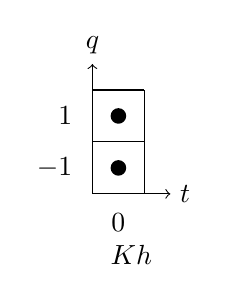
\begin{tikzpicture}[scale=.66]
  \draw[->] (0,0) -- (1.5,0) node[right] {$t$};
  \draw[->] (0,0) -- (0,2.5) node[above] {$q$};
  \draw[step=1] (0,0) grid (1,2);
  \draw (0.750,-0.8) node[below] {$Kh$};
  \draw (0.5,-.2) node[below] {$0$};
  \draw (-.2,0.5) node[left] {$-1$};
  \draw (-.2,1.5) node[left] {$1$};
  \fill (0.5, 0.5) circle (.15);
  \fill (0.5, 1.5) circle (.15);
\end{tikzpicture}  \qquad Kh = $Kh(\verb~T(2,3)~; \verb~Z2~)$:\\
$\text{rank} Kh = 6$\\
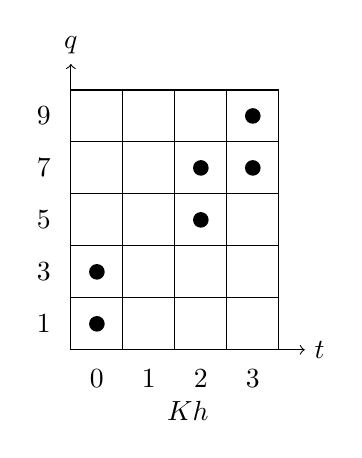
\begin{tikzpicture}[scale=.66]
  \draw[->] (0,0) -- (4.5,0) node[right] {$t$};
  \draw[->] (0,0) -- (0,5.5) node[above] {$q$};
  \draw[step=1] (0,0) grid (4,5);
  \draw (2.250,-0.8) node[below] {$Kh$};
  \draw (0.5,-.2) node[below] {$0$};
  \draw (1.5,-.2) node[below] {$1$};
  \draw (2.5,-.2) node[below] {$2$};
  \draw (3.5,-.2) node[below] {$3$};
  \draw (-.2,0.5) node[left] {$1$};
  \draw (-.2,1.5) node[left] {$3$};
  \draw (-.2,2.5) node[left] {$5$};
  \draw (-.2,3.5) node[left] {$7$};
  \draw (-.2,4.5) node[left] {$9$};
  \fill (0.5, 0.5) circle (.15);
  \fill (0.5, 1.5) circle (.15);
  \fill (2.5, 2.5) circle (.15);
  \fill (2.5, 3.5) circle (.15);
  \fill (3.5, 3.5) circle (.15);
  \fill (3.5, 4.5) circle (.15);
\end{tikzpicture}
  
Kh = $Kh(\verb~T(2,5)~; \verb~Z2~)$:\\
$\text{rank} Kh = 10$\\
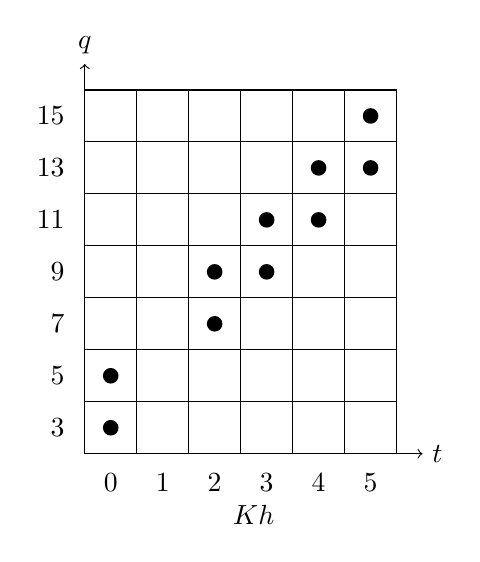
\begin{tikzpicture}[scale=.66]
  \draw[->] (0,0) -- (6.5,0) node[right] {$t$};
  \draw[->] (0,0) -- (0,7.5) node[above] {$q$};
  \draw[step=1] (0,0) grid (6,7);
  \draw (3.250,-0.8) node[below] {$Kh$};
  \draw (0.5,-.2) node[below] {$0$};
  \draw (1.5,-.2) node[below] {$1$};
  \draw (2.5,-.2) node[below] {$2$};
  \draw (3.5,-.2) node[below] {$3$};
  \draw (4.5,-.2) node[below] {$4$};
  \draw (5.5,-.2) node[below] {$5$};
  \draw (-.2,0.5) node[left] {$3$};
  \draw (-.2,1.5) node[left] {$5$};
  \draw (-.2,2.5) node[left] {$7$};
  \draw (-.2,3.5) node[left] {$9$};
  \draw (-.2,4.5) node[left] {$11$};
  \draw (-.2,5.5) node[left] {$13$};
  \draw (-.2,6.5) node[left] {$15$};
  \fill (0.5, 0.5) circle (.15);
  \fill (0.5, 1.5) circle (.15);
  \fill (2.5, 2.5) circle (.15);
  \fill (2.5, 3.5) circle (.15);
  \fill (3.5, 3.5) circle (.15);
  \fill (3.5, 4.5) circle (.15);
  \fill (4.5, 4.5) circle (.15);
  \fill (4.5, 5.5) circle (.15);
  \fill (5.5, 5.5) circle (.15);
  \fill (5.5, 6.5) circle (.15);
\end{tikzpicture}

Kh = $Kh(\verb~T(2,7)~; \verb~Z2~)$:\\
$\text{rank} Kh = 14$\\
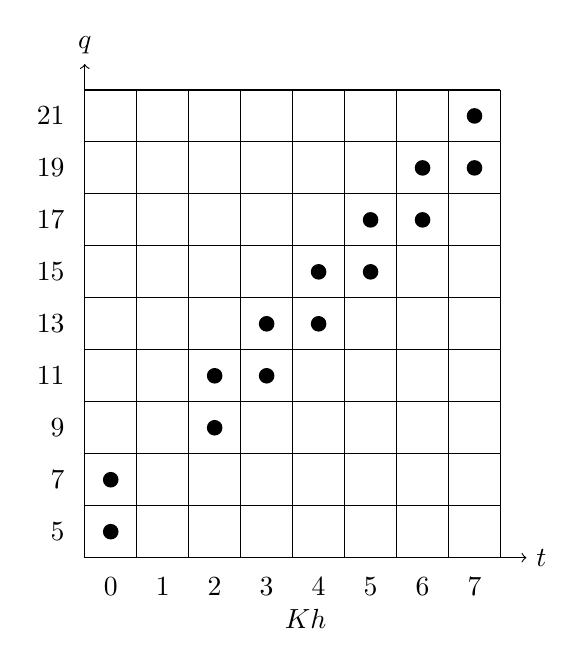
\begin{tikzpicture}[scale=.66]
  \draw[->] (0,0) -- (8.5,0) node[right] {$t$};
  \draw[->] (0,0) -- (0,9.5) node[above] {$q$};
  \draw[step=1] (0,0) grid (8,9);
  \draw (4.250,-0.8) node[below] {$Kh$};
  \draw (0.5,-.2) node[below] {$0$};
  \draw (1.5,-.2) node[below] {$1$};
  \draw (2.5,-.2) node[below] {$2$};
  \draw (3.5,-.2) node[below] {$3$};
  \draw (4.5,-.2) node[below] {$4$};
  \draw (5.5,-.2) node[below] {$5$};
  \draw (6.5,-.2) node[below] {$6$};
  \draw (7.5,-.2) node[below] {$7$};
  \draw (-.2,0.5) node[left] {$5$};
  \draw (-.2,1.5) node[left] {$7$};
  \draw (-.2,2.5) node[left] {$9$};
  \draw (-.2,3.5) node[left] {$11$};
  \draw (-.2,4.5) node[left] {$13$};
  \draw (-.2,5.5) node[left] {$15$};
  \draw (-.2,6.5) node[left] {$17$};
  \draw (-.2,7.5) node[left] {$19$};
  \draw (-.2,8.5) node[left] {$21$};
  \fill (0.5, 0.5) circle (.15);
  \fill (0.5, 1.5) circle (.15);
  \fill (2.5, 2.5) circle (.15);
  \fill (2.5, 3.5) circle (.15);
  \fill (3.5, 3.5) circle (.15);
  \fill (3.5, 4.5) circle (.15);
  \fill (4.5, 4.5) circle (.15);
  \fill (4.5, 5.5) circle (.15);
  \fill (5.5, 5.5) circle (.15);
  \fill (5.5, 6.5) circle (.15);
  \fill (6.5, 6.5) circle (.15);
  \fill (6.5, 7.5) circle (.15);
  \fill (7.5, 7.5) circle (.15);
  \fill (7.5, 8.5) circle (.15);
\end{tikzpicture}

Kh = $Kh(\verb~T(2,9)~; \verb~Z2~)$:\\
$\text{rank} Kh = 18$\\
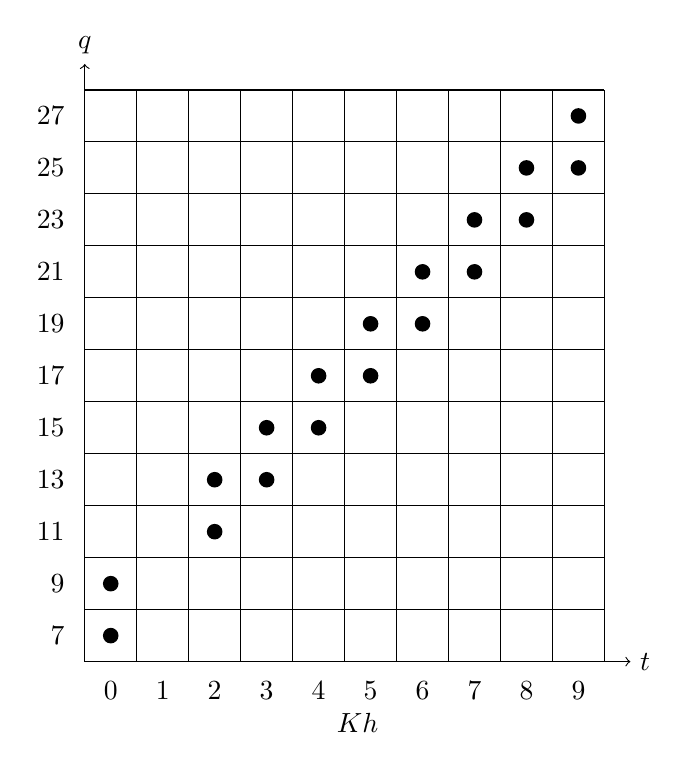
\begin{tikzpicture}[scale=.66]
  \draw[->] (0,0) -- (10.5,0) node[right] {$t$};
  \draw[->] (0,0) -- (0,11.5) node[above] {$q$};
  \draw[step=1] (0,0) grid (10,11);
  \draw (5.250,-0.8) node[below] {$Kh$};
  \draw (0.5,-.2) node[below] {$0$};
  \draw (1.5,-.2) node[below] {$1$};
  \draw (2.5,-.2) node[below] {$2$};
  \draw (3.5,-.2) node[below] {$3$};
  \draw (4.5,-.2) node[below] {$4$};
  \draw (5.5,-.2) node[below] {$5$};
  \draw (6.5,-.2) node[below] {$6$};
  \draw (7.5,-.2) node[below] {$7$};
  \draw (8.5,-.2) node[below] {$8$};
  \draw (9.5,-.2) node[below] {$9$};
  \draw (-.2,0.5) node[left] {$7$};
  \draw (-.2,1.5) node[left] {$9$};
  \draw (-.2,2.5) node[left] {$11$};
  \draw (-.2,3.5) node[left] {$13$};
  \draw (-.2,4.5) node[left] {$15$};
  \draw (-.2,5.5) node[left] {$17$};
  \draw (-.2,6.5) node[left] {$19$};
  \draw (-.2,7.5) node[left] {$21$};
  \draw (-.2,8.5) node[left] {$23$};
  \draw (-.2,9.5) node[left] {$25$};
  \draw (-.2,10.5) node[left] {$27$};
  \fill (0.5, 0.5) circle (.15);
  \fill (0.5, 1.5) circle (.15);
  \fill (2.5, 2.5) circle (.15);
  \fill (2.5, 3.5) circle (.15);
  \fill (3.5, 3.5) circle (.15);
  \fill (3.5, 4.5) circle (.15);
  \fill (4.5, 4.5) circle (.15);
  \fill (4.5, 5.5) circle (.15);
  \fill (5.5, 5.5) circle (.15);
  \fill (5.5, 6.5) circle (.15);
  \fill (6.5, 6.5) circle (.15);
  \fill (6.5, 7.5) circle (.15);
  \fill (7.5, 7.5) circle (.15);
  \fill (7.5, 8.5) circle (.15);
  \fill (8.5, 8.5) circle (.15);
  \fill (8.5, 9.5) circle (.15);
  \fill (9.5, 9.5) circle (.15);
  \fill (9.5, 10.5) circle (.15);
\end{tikzpicture}

Kh = $Kh(\verb~T(2,11)~; \verb~Z2~)$:\\
$\text{rank} Kh = 22$\\
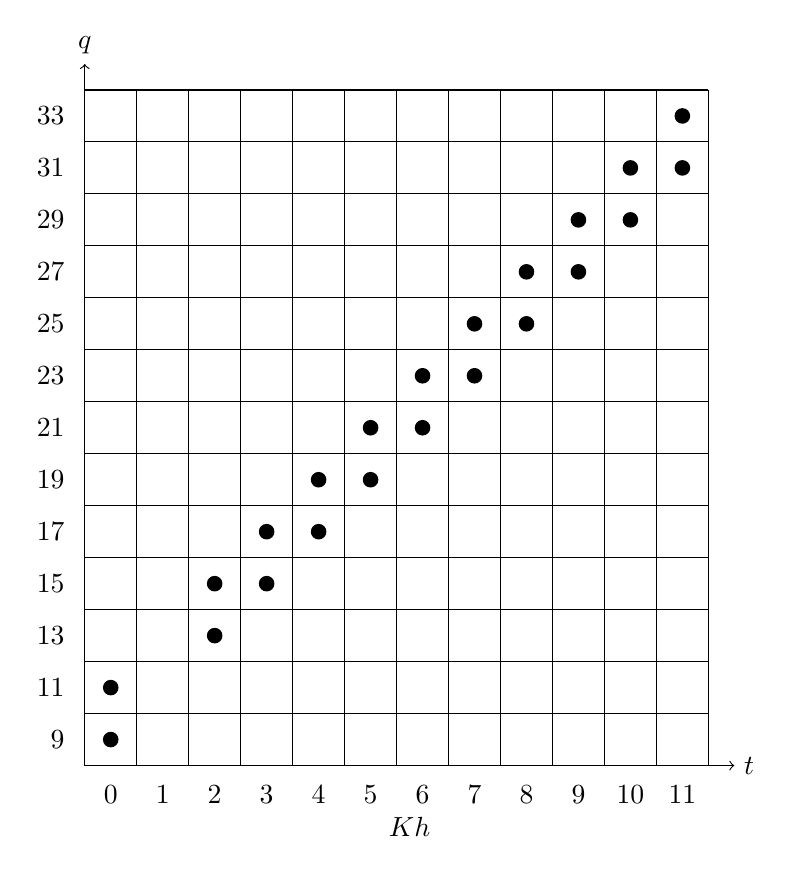
\begin{tikzpicture}[scale=.66]
  \draw[->] (0,0) -- (12.5,0) node[right] {$t$};
  \draw[->] (0,0) -- (0,13.5) node[above] {$q$};
  \draw[step=1] (0,0) grid (12,13);
  \draw (6.250,-0.8) node[below] {$Kh$};
  \draw (0.5,-.2) node[below] {$0$};
  \draw (1.5,-.2) node[below] {$1$};
  \draw (2.5,-.2) node[below] {$2$};
  \draw (3.5,-.2) node[below] {$3$};
  \draw (4.5,-.2) node[below] {$4$};
  \draw (5.5,-.2) node[below] {$5$};
  \draw (6.5,-.2) node[below] {$6$};
  \draw (7.5,-.2) node[below] {$7$};
  \draw (8.5,-.2) node[below] {$8$};
  \draw (9.5,-.2) node[below] {$9$};
  \draw (10.5,-.2) node[below] {$10$};
  \draw (11.5,-.2) node[below] {$11$};
  \draw (-.2,0.5) node[left] {$9$};
  \draw (-.2,1.5) node[left] {$11$};
  \draw (-.2,2.5) node[left] {$13$};
  \draw (-.2,3.5) node[left] {$15$};
  \draw (-.2,4.5) node[left] {$17$};
  \draw (-.2,5.5) node[left] {$19$};
  \draw (-.2,6.5) node[left] {$21$};
  \draw (-.2,7.5) node[left] {$23$};
  \draw (-.2,8.5) node[left] {$25$};
  \draw (-.2,9.5) node[left] {$27$};
  \draw (-.2,10.5) node[left] {$29$};
  \draw (-.2,11.5) node[left] {$31$};
  \draw (-.2,12.5) node[left] {$33$};
  \fill (0.5, 0.5) circle (.15);
  \fill (0.5, 1.5) circle (.15);
  \fill (2.5, 2.5) circle (.15);
  \fill (2.5, 3.5) circle (.15);
  \fill (3.5, 3.5) circle (.15);
  \fill (3.5, 4.5) circle (.15);
  \fill (4.5, 4.5) circle (.15);
  \fill (4.5, 5.5) circle (.15);
  \fill (5.5, 5.5) circle (.15);
  \fill (5.5, 6.5) circle (.15);
  \fill (6.5, 6.5) circle (.15);
  \fill (6.5, 7.5) circle (.15);
  \fill (7.5, 7.5) circle (.15);
  \fill (7.5, 8.5) circle (.15);
  \fill (8.5, 8.5) circle (.15);
  \fill (8.5, 9.5) circle (.15);
  \fill (9.5, 9.5) circle (.15);
  \fill (9.5, 10.5) circle (.15);
  \fill (10.5, 10.5) circle (.15);
  \fill (10.5, 11.5) circle (.15);
  \fill (11.5, 11.5) circle (.15);
  \fill (11.5, 12.5) circle (.15);
\end{tikzpicture}

Kh = $Kh(\verb~T(2,13)~; \verb~Z2~)$:\\
$\text{rank} Kh = 26$\\
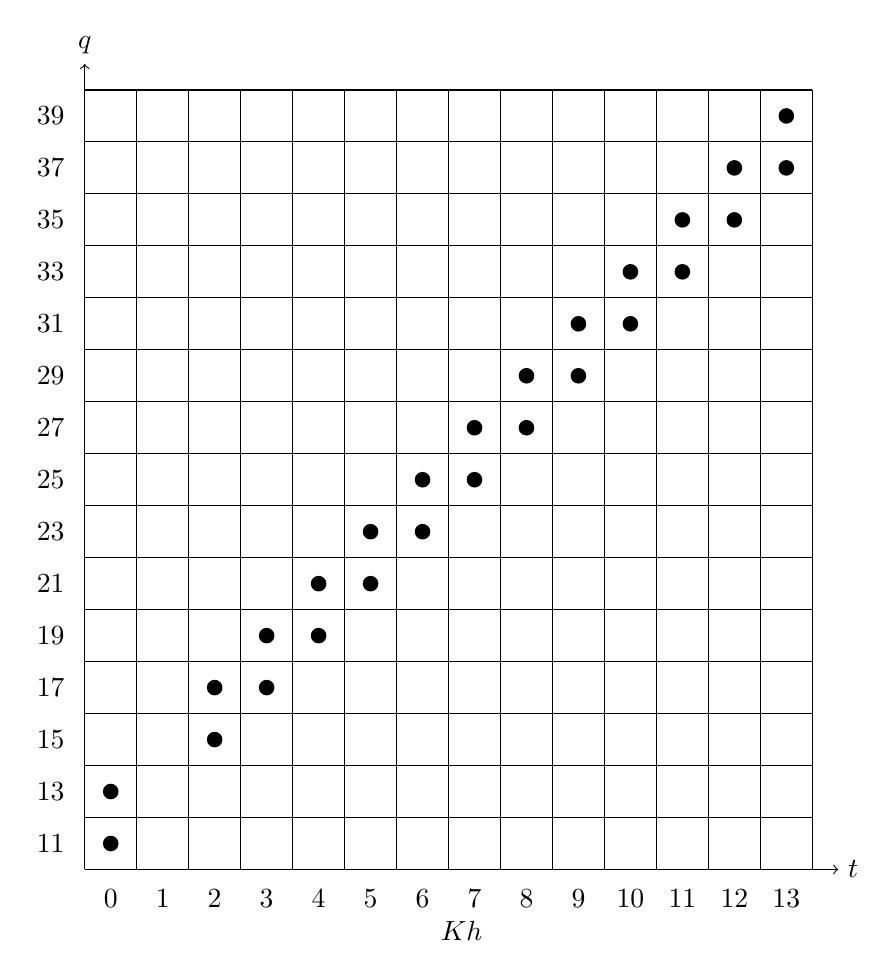
\begin{tikzpicture}[scale=.66]
  \draw[->] (0,0) -- (14.5,0) node[right] {$t$};
  \draw[->] (0,0) -- (0,15.5) node[above] {$q$};
  \draw[step=1] (0,0) grid (14,15);
  \draw (7.250,-0.8) node[below] {$Kh$};
  \draw (0.5,-.2) node[below] {$0$};
  \draw (1.5,-.2) node[below] {$1$};
  \draw (2.5,-.2) node[below] {$2$};
  \draw (3.5,-.2) node[below] {$3$};
  \draw (4.5,-.2) node[below] {$4$};
  \draw (5.5,-.2) node[below] {$5$};
  \draw (6.5,-.2) node[below] {$6$};
  \draw (7.5,-.2) node[below] {$7$};
  \draw (8.5,-.2) node[below] {$8$};
  \draw (9.5,-.2) node[below] {$9$};
  \draw (10.5,-.2) node[below] {$10$};
  \draw (11.5,-.2) node[below] {$11$};
  \draw (12.5,-.2) node[below] {$12$};
  \draw (13.5,-.2) node[below] {$13$};
  \draw (-.2,0.5) node[left] {$11$};
  \draw (-.2,1.5) node[left] {$13$};
  \draw (-.2,2.5) node[left] {$15$};
  \draw (-.2,3.5) node[left] {$17$};
  \draw (-.2,4.5) node[left] {$19$};
  \draw (-.2,5.5) node[left] {$21$};
  \draw (-.2,6.5) node[left] {$23$};
  \draw (-.2,7.5) node[left] {$25$};
  \draw (-.2,8.5) node[left] {$27$};
  \draw (-.2,9.5) node[left] {$29$};
  \draw (-.2,10.5) node[left] {$31$};
  \draw (-.2,11.5) node[left] {$33$};
  \draw (-.2,12.5) node[left] {$35$};
  \draw (-.2,13.5) node[left] {$37$};
  \draw (-.2,14.5) node[left] {$39$};
  \fill (0.5, 0.5) circle (.15);
  \fill (0.5, 1.5) circle (.15);
  \fill (2.5, 2.5) circle (.15);
  \fill (2.5, 3.5) circle (.15);
  \fill (3.5, 3.5) circle (.15);
  \fill (3.5, 4.5) circle (.15);
  \fill (4.5, 4.5) circle (.15);
  \fill (4.5, 5.5) circle (.15);
  \fill (5.5, 5.5) circle (.15);
  \fill (5.5, 6.5) circle (.15);
  \fill (6.5, 6.5) circle (.15);
  \fill (6.5, 7.5) circle (.15);
  \fill (7.5, 7.5) circle (.15);
  \fill (7.5, 8.5) circle (.15);
  \fill (8.5, 8.5) circle (.15);
  \fill (8.5, 9.5) circle (.15);
  \fill (9.5, 9.5) circle (.15);
  \fill (9.5, 10.5) circle (.15);
  \fill (10.5, 10.5) circle (.15);
  \fill (10.5, 11.5) circle (.15);
  \fill (11.5, 11.5) circle (.15);
  \fill (11.5, 12.5) circle (.15);
  \fill (12.5, 12.5) circle (.15);
  \fill (12.5, 13.5) circle (.15);
  \fill (13.5, 13.5) circle (.15);
  \fill (13.5, 14.5) circle (.15);
\end{tikzpicture}

Kh = $Kh(\verb~T(3,4)~; \verb~Z2~)$:\\
$\text{rank} Kh = 10$\\
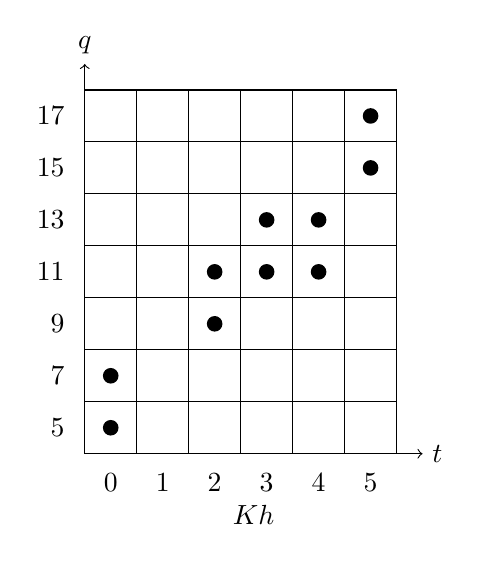
\begin{tikzpicture}[scale=.66]
  \draw[->] (0,0) -- (6.5,0) node[right] {$t$};
  \draw[->] (0,0) -- (0,7.5) node[above] {$q$};
  \draw[step=1] (0,0) grid (6,7);
  \draw (3.250,-0.8) node[below] {$Kh$};
  \draw (0.5,-.2) node[below] {$0$};
  \draw (1.5,-.2) node[below] {$1$};
  \draw (2.5,-.2) node[below] {$2$};
  \draw (3.5,-.2) node[below] {$3$};
  \draw (4.5,-.2) node[below] {$4$};
  \draw (5.5,-.2) node[below] {$5$};
  \draw (-.2,0.5) node[left] {$5$};
  \draw (-.2,1.5) node[left] {$7$};
  \draw (-.2,2.5) node[left] {$9$};
  \draw (-.2,3.5) node[left] {$11$};
  \draw (-.2,4.5) node[left] {$13$};
  \draw (-.2,5.5) node[left] {$15$};
  \draw (-.2,6.5) node[left] {$17$};
  \fill (0.5, 0.5) circle (.15);
  \fill (0.5, 1.5) circle (.15);
  \fill (2.5, 2.5) circle (.15);
  \fill (2.5, 3.5) circle (.15);
  \fill (3.5, 3.5) circle (.15);
  \fill (3.5, 4.5) circle (.15);
  \fill (4.5, 3.5) circle (.15);
  \fill (4.5, 4.5) circle (.15);
  \fill (5.5, 5.5) circle (.15);
  \fill (5.5, 6.5) circle (.15);
\end{tikzpicture}

Kh = $Kh(\verb~T(3,5)~; \verb~Z2~)$:\\
$\text{rank} Kh = 14$\\
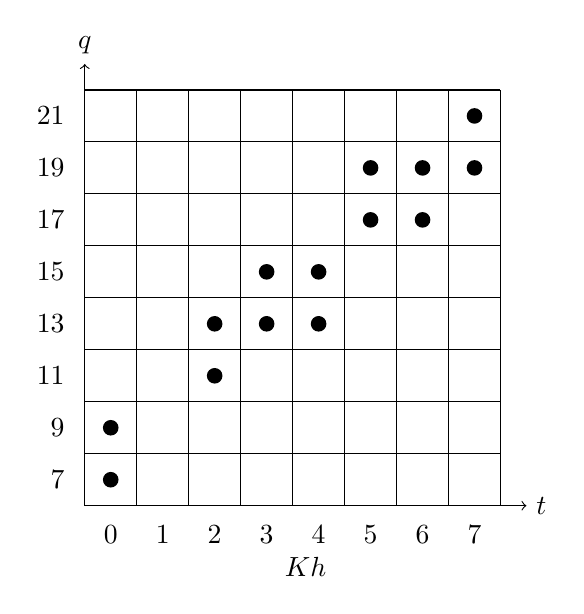
\begin{tikzpicture}[scale=.66]
  \draw[->] (0,0) -- (8.5,0) node[right] {$t$};
  \draw[->] (0,0) -- (0,8.5) node[above] {$q$};
  \draw[step=1] (0,0) grid (8,8);
  \draw (4.250,-0.8) node[below] {$Kh$};
  \draw (0.5,-.2) node[below] {$0$};
  \draw (1.5,-.2) node[below] {$1$};
  \draw (2.5,-.2) node[below] {$2$};
  \draw (3.5,-.2) node[below] {$3$};
  \draw (4.5,-.2) node[below] {$4$};
  \draw (5.5,-.2) node[below] {$5$};
  \draw (6.5,-.2) node[below] {$6$};
  \draw (7.5,-.2) node[below] {$7$};
  \draw (-.2,0.5) node[left] {$7$};
  \draw (-.2,1.5) node[left] {$9$};
  \draw (-.2,2.5) node[left] {$11$};
  \draw (-.2,3.5) node[left] {$13$};
  \draw (-.2,4.5) node[left] {$15$};
  \draw (-.2,5.5) node[left] {$17$};
  \draw (-.2,6.5) node[left] {$19$};
  \draw (-.2,7.5) node[left] {$21$};
  \fill (0.5, 0.5) circle (.15);
  \fill (0.5, 1.5) circle (.15);
  \fill (2.5, 2.5) circle (.15);
  \fill (2.5, 3.5) circle (.15);
  \fill (3.5, 3.5) circle (.15);
  \fill (3.5, 4.5) circle (.15);
  \fill (4.5, 3.5) circle (.15);
  \fill (4.5, 4.5) circle (.15);
  \fill (5.5, 5.5) circle (.15);
  \fill (5.5, 6.5) circle (.15);
  \fill (6.5, 5.5) circle (.15);
  \fill (6.5, 6.5) circle (.15);
  \fill (7.5, 6.5) circle (.15);
  \fill (7.5, 7.5) circle (.15);
\end{tikzpicture}
\end{center}
\fussy

If you wanted to \emph{save the output} from option flag ``khplainout'', then one simple and direct manner is to ``pipe'' the screen output with the symbol ``\verb|>|'' at the Command prompt and specify the target file you'd want to save the output.  For example, for the Torus knot $T(2,5)$, saving into the file \verb|kh_T0205| in the directory above the current working directory,
\[
\verb|./kk khplainout -v ``T(2,5)'' > ../kh_T0205|
\]
I've done this for all torus knots of less than 14 crossings and saved the output and placed them in the github repository \verb|qsApoly| so others can have access to the Khovanov homology computation outputs readily; they are named files \verb|kh_T0203|, \verb|kh_T0205|, $\dots$ in \verb|kk_kh_output|.  

If you don't want to do this one-by-one, but a batch of these, one at a time, see the Python script \verb|kk_kh_batch.py|, which you can run directly by typing at the command prompt \verb|python kk_kh_batch.py| or manually, by opening up an interactive shell (i.e. \verb|python -i kk_kh_batch.py|) and then running manually the Python function \verb|direct_output|.  

To ``clean'' or ``scrape'' the text (strings) of ``categorified'' Jones polynomial, to get it ready to use for \verb|Sage Math|, I provide the file \verb|kh_scrape.py|.  It contains the function \verb|scrape_file| that will take a file containing a \emph{single} categorified Jones polynomial and output a ``cleaned up'' text (string) for the polynomial, in a Python dictionary, that can be used in Sage Math (just then apply the Sage Math function \verb|sage_eval|).  For example:
\begin{lstlisting}
from kh_scrape import scrape_file
Qkh.<t,q> = PolynomialRing(RationalField(),2)
T0203stf = scrape_file('kh_T0203')
T0203poly = sage_eval( T0203stf['poly'], locals={'x1':t,'x2':q} )
T0203poly.substitute(t=-1) # for some reason, subs doesn't work in this case
\end{lstlisting}
Also, from running \verb|kh_scrape.py| and function \verb|scrape_bat| in \emph{Sage Math} (make sure you're in the appropriate working directory)
\begin{lstlisting}
sage: from kh_scrape import scrape_bat
sage: Tknots14 = scrape_bat('khTknotsless14')
sage: Tknots14sage = [ sage_eval(line, locals={'x1':t,'x2':q}) for line in Tknots14 ]
sage: for K in Tknots14sage:
....:           print latex(K)
\end{lstlisting}
Then you'll have all the torus knots categorified Jones polynomials from Khovanov Homology in a single list ``Tknots14sage'' (but you'll have to manually keep track of which entry corresponds to which torus knot).  

The result of printing with \verb|latex| command in the last command immediately above is this table of ``categorified'' Jones polynomials from Khovanov Homology (source:\verb|knotkit|)

\begin{landscape}
\begin{center}
\begin{tabular}{l c}
  K & J(K;t,q) \\ \hline 
  $T(2,1)$ & $\frac{q^{2} + 1}{q}$ \\
  $T(2,3)$ & $t^{3} q^{9} + t^{3} q^{7} + t^{2} q^{7} + t^{2} q^{5} + q^{3} + q$ \\
  $T(2,5)$ & $t^{5} q^{15} + t^{5} q^{13} + t^{4} q^{13} + t^{4} q^{11} + t^{3} q^{11} + t^{3} q^{9} + t^{2} q^{9} + t^{2} q^{7} + q^{5} + q^{3}$ \\
  $T(2,7)$ & $t^{7} q^{21} + t^{7} q^{19} + t^{6} q^{19} + t^{6} q^{17} + t^{5} q^{17} + t^{5} q^{15} + t^{4} q^{15} + t^{4} q^{13} + t^{3} q^{13} + t^{3} q^{11} + t^{2} q^{11} + t^{2} q^{9} + q^{7} + q^{5}$  \\

\end{tabular}
%\label{table:JonespolysSnapPy}
\end{center} \qquad \\

For  $T(2,9)$,
\begin{dmath} 
  t^{9} q^{27} + t^{9} q^{25} + t^{8} q^{25} + t^{8} q^{23} + t^{7} q^{23} + t^{7} q^{21} + t^{6} q^{21} + t^{6} q^{19} + t^{5} q^{19} + t^{5} q^{17} + t^{4} q^{17} + t^{4} q^{15} + t^{3} q^{15} + t^{3} q^{13} + t^{2} q^{13} + t^{2} q^{11} + q^{9} + q^{7} 
\end{dmath}

For   $T(2,11)$, 
\begin{dmath}
  t^{11} q^{33} + t^{11} q^{31} + t^{10} q^{31} + t^{10} q^{29} + t^{9} q^{29} + t^{9} q^{27} + t^{8} q^{27} + t^{8} q^{25} + t^{7} q^{25} + t^{7} q^{23} + t^{6} q^{23} + t^{6} q^{21} + t^{5} q^{21} + t^{5} q^{19} + t^{4} q^{19} + t^{4} q^{17} + t^{3} q^{17} + t^{3} q^{15} + t^{2} q^{15} + t^{2} q^{13} + q^{11} + q^{9}
\end{dmath}



For  $T(2,13)$,
\begin{dmath} t^{13} q^{39} + t^{13} q^{37} + t^{12} q^{37} + t^{12} q^{35} + t^{11} q^{35} + t^{11} q^{33} + t^{10} q^{33} + t^{10} q^{31} + t^{9} q^{31} + t^{9} q^{29} + t^{8} q^{29} + t^{8} q^{27} + t^{7} q^{27} + t^{7} q^{25} + t^{6} q^{25} + t^{6} q^{23} + t^{5} q^{23} + t^{5} q^{21} + t^{4} q^{21} + t^{4} q^{19} + t^{3} q^{19} + t^{3} q^{17} + t^{2} q^{17} + t^{2} q^{15} + q^{13} + q^{11} \end{dmath} 


For $T(3,4)$,
\begin{dmath}
t^{5} q^{17} + t^{5} q^{15} + t^{4} q^{13} + t^{3} q^{13} + t^{4} q^{11} + t^{3} q^{11} + t^{2} q^{11} + t^{2} q^{9} + q^{7} + q^{5}
\end{dmath}

For, $T(3,5)$,
\begin{dmath}
t^{7} q^{21} + t^{7} q^{19} + t^{6} q^{19} + t^{5} q^{19} + t^{6} q^{17} + t^{5} q^{17} + t^{4} q^{15} + t^{3} q^{15} + t^{4} q^{13} + t^{3} q^{13} + t^{2} q^{13} + t^{2} q^{11} + q^{9} + q^{7}
\end{dmath}


\end{landscape}




The miracle is that if one sets $t=-1$ in the above categorified Jones polynomials, $J(K;t,q)$, then $J(K;t=-1,q) = J(K,q)$, where $J(K,q)$ are the Jones polynomials (modulo conventions), from Table \ref{table:JonespolysSnapPy}!

To show this, keep in mind that for the categorified Jones polynomials, one must \emph{normalize} to the ``unknot'' which in this case is the $T(2,1)$ torus knot, after setting $t=-1$ (or before? that's my question; please let me know what ``dividing'' by the unknot means in both cases):
\begin{lstlisting}
sage: normTknots14sage = [K/Tknots14sage[0] for K in Tknots14sage]

# Compare Jones polynomials from SnaPy to Jones polynomials from decategorified Khovanov Homology:
sage: x = var('x')
sage: for i in range(1,len(TKNOTS14SNAP)):
          SnaPyvskh = TKNOTS14SNAP[TKNOTSLIST14[i]].jones_poly().subs(q=x) == 
                       normTknots14sage[i].subs(t=-1).subs(q=sqrt(x))
          print bool( SnaPyvskh )

sage: print "If all True, then J(K;t=-1,q) = J(K;q)!"
\end{lstlisting}  
and indeed it does.  

Note that for some reason, the Jones polynomial for $T(2,1)$ of \emph{SnaPy} produces this error: 
\begin{lstlisting}
sage: TKNOTS14SNAP[(2,1)].jones_poly()
# stuff
IndexError: list index out of range
\end{lstlisting}

EY: 20160224: My immediate question is this: what's the convention or normalization that results in SnaPy outputting the Jones polynomial for the torus knots, say $T(2,3)$ trefoil knot, to be
\[
-q^{4} + q^{3} + q
\]
vs. the Jones polynomial that results from Khovanov homology, after setting $t=-1$, for the trefoil:
\[
- q^{8} + q^{6} + q^{2}
\]
The latter expression is found on pp. 339 of Bar-Natan's (nicely, pedagogically-friendly) review artcle \cite{DBar-Natan2002}

\section{Exploring the Jones Polynomial and Khovanov Homology: Unanswered Avenues}

Armed with our categorified Jones polynomials and Sage Math, there are a number of modules (functions) that can be explored, as seen if one does the \verb|dir()| command on a polynomial (e.g. \verb|dir(Tknots14sage[1])|).  

For instance, consider 
\begin{lstlisting}
  sage: Tknots14sage[1].gradient() # T(2,3)
  [3*t^2*q^9 + 3*t^2*q^7 + 2*t*q^7 + 2*t*q^5,
    9*t^3*q^8 + 7*t^3*q^6 + 7*t^2*q^6 + 5*t^2*q^4 + 3*q^2 + 1]
\end{lstlisting}
which is $\frac{ \partial }{ \partial t} J(T(2,3);t,q)$ and $\frac{ \partial }{ \partial q} J(T(2,3);t,q)$.  Are there any relationships we can discover between the categorified Jones polynomial and its partial(s) (derivatives)?

One can also use the Sage Math module \verb|newton_polytope| to obtain the Newton Polytope immediately.  One does the Newton Polytope tell us about categorified Jones polynomials?

Also, there are many Sage Math modules associated with \verb|newton_polytope| (i.e. do e.g. \verb|dir(Tknots14sage[1].newton_polytope())|), such as \verb|face_lattice|:
\begin{lstlisting}
sage: Tknots14sage[1].newton_polytope().face_lattice().list()
[<>, <0>, <1>, <2>, <3>, <1,2>, <0,1>, <0,3>, <2,3>, <0,1,2,3>]
sage: Tknots14sage[7].newton_polytope().face_lattice().list()
[<>, <0>, <1>, <2>, <3>, <4>, <1,2>, <0,1>, <0,4>, <3,4>, <2,3>, <0,1,2,3,4>]
\end{lstlisting}
So the face lattice of a $T(2,2j+1)$ torus knot, $j=1\dots 6$, is different from the family of torus knots $T(3,4)$ and $T(3,5)$.  What does that mean?  

This reference page might help with polytopes: \href{http://doc.sagemath.org/html/en/reference/geometry/sage/geometry/polyhedron/face.html}{A class to keep information about faces of a polyhedron}

Something else one could try to do is to repeat Witten's celebrated computation of the Jones polynomial from Chern-Simons theory \cite{Witten:1988hf} in \emph{Sage Math}.  This would entail an understanding, a grasp, of the Weyl group, in this case, $SU(2)$.  I tried looking up topics on the Weyl group and Weyl character in Sage Math (cf. \href{http://doc.sagemath.org/html/en/reference/combinat/sage/combinat/root_system/weyl_group.html}{Weyl Group}, \href{https://www.math.ucdavis.edu/~anne/SQ2014/thematic_tutorials/lie/weyl_character_ring.html\#slvsgl}{SL versus GL})



\subsection{Installation of SnapPy}\label{SubSec:InstallSnapPy}

\subsubsection{Mac OS X Installation of SnapPy}

First, one should simply download \href{https://bitbucket.org/t3m/snappy/downloads/SnapPy.dmg}{SnapPy.dmg}, and then double-click the .dmg file and then drag-and-drog the SnapPy icon into the Applications Folder \footnote{cf. \href{http://www.math.uic.edu/t3m/SnapPy/installing.html}{Installing SnapPy}}.  

However, one would like to take advantage of its integration with \verb|Sage Math| and so here's how to install SnapPy into \verb|Sage|.  

\begin{enumerate}
\item Go to or \verb|cd| into the directory where the main program \verb|sage| is in; for example, the directory that \verb|sage|, the \emph{executable file} is in, is 
\[
\verb|/Applications/SageMath-6.10.app/Contents/Resources/sage|
\]
where \verb|sage| here is a \emph{directory}.  
\item Make sure you have \verb|pip| installed and do this command:
\[
\verb|./sage -pip install --no-use-wheel snappy|
\]
cf. \url{http://www.math.uic.edu/t3m/SnapPy/installing.html\#sage}.  It should successfully install.
\end{enumerate}




\begin{thebibliography}{9}

\bibitem{MCullerNDunfieldJWeeks}
M. Culler, N. M. Dunfield, and J. R. Weeks, SnapPy, a computer program for studying the geometry and topology of 3-manifolds, \url{http://snappy.computop.org}

\bibitem{DBar-Natan2002}
Dror Bar-Natan. ``On Khovanov’s categorification of the Jones polynomial.'' \textbf{Algebraic \& Geometric Topology}.  Volume 2 (2002) 337–370.  \href{http://arxiv.org/abs/math/0201043}{arXiv:math/0201043v3 [math.QA]}

%\cite{Witten:1988hf}
\bibitem{Witten:1988hf} 
  E.~Witten,
  %``Quantum Field Theory and the Jones Polynomial,''
  Commun.\ Math.\ Phys.\  {\bf 121}, 351 (1989).
  doi:10.1007/BF01217730
  %%CITATION = doi:10.1007/BF01217730;%%
  %2286 citations counted in INSPIRE as of 24 Feb 2016

\end{thebibliography}

\end{document}
